\documentclass[a4paper,12pt]{article}
\usepackage[fleqn]{amsmath}
\usepackage{amssymb}
\usepackage{graphicx}
\graphicspath{ {./images/} }
\begin{document}

\title{Data Processing}	
\author{Edward Jex}
\maketitle
\section*{Different Types of Data}
\begin{itemize}
	\item Categorical - Generally not numerical.
	\item Discrete - Only certain values, normally integers. 
	\item Continuous - Numerical, real values.
	\item Ranked - Numerical, ordered.
\end{itemize}

\subsection*{Categorical data}
For categorical data, the most common summary measure of our data is the modal class. This is the class with the highest frequency. 
Diagrams:
\begin{itemize}
	\item Bar chart 
	\item Pie chart
	\item Pictogram 
	\item Pot chart 
\end{itemize} 

\subsection*{Ranked Data}
If our data is ranked, we normally use stem and leaf diagrams or box plots to represent the data. 

\subsubsection*{Stem and Leaf Diagrams} 
Example:\\
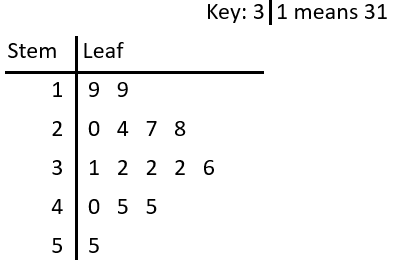
\includegraphics[scale=0.7]{StemAndLeafDiagram}\\
Note: includes repeats, only a single digit on the right.\\\\

For ranked data, we often use the median, lower and upper quartiles as our summary measures. 
\begin{itemize}
	\item The median value ($Q_2$) - The middle number 
	\item The lower quartile ($Q_1$) - The middle number of the lower half
	\item The upper quartile ($Q_3$) - The middle number of the upper half
\end{itemize}
If the number of data-points is off, you just take the middle number. If it is even, take the average between the two middle numbers and when calculating the quartiles, include the middle.

\subsubsection*{Box Plots} 
The five key numbers can be shown on a simple diagram known as a box-and-whisker plot.\\
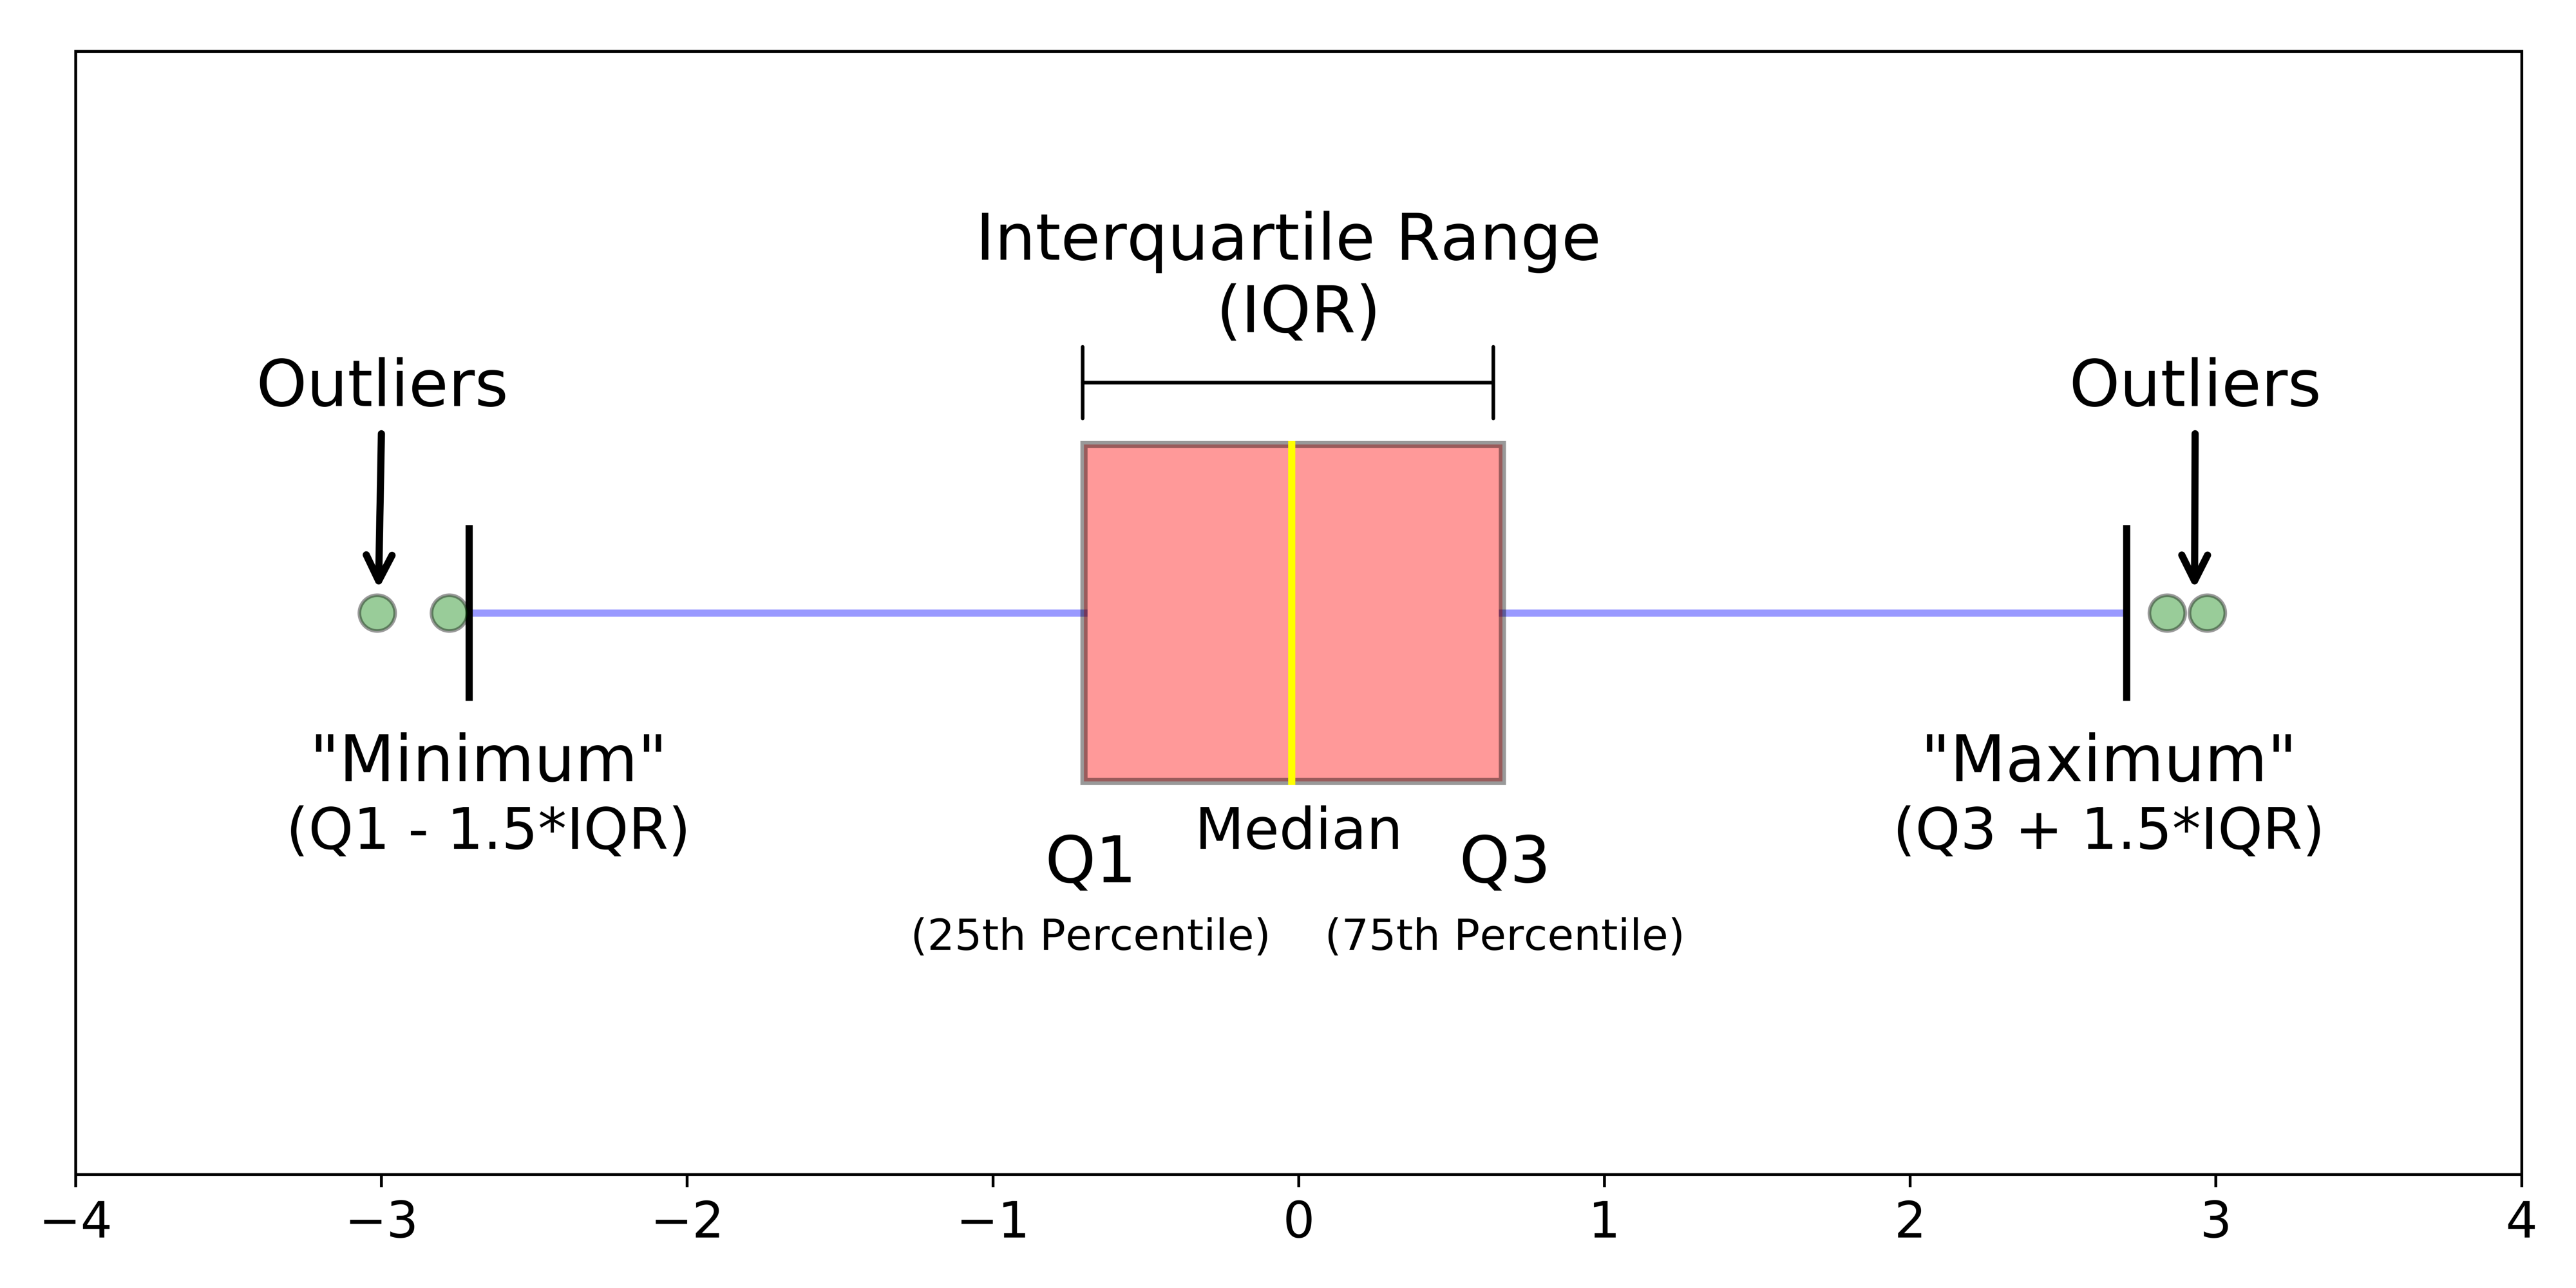
\includegraphics[scale=0.07]{BoxPlot}\\

\subsection*{Outliers}
We can say that a data-point is an outlier if the data-point is more than $1.5 \times$ IQR beyond or below the lower or upper quartiles. 
\section*{Product-Moment Correlation Coefficient}
The PMCC measures hot close the data is to a straight line. \\
$r = \frac{S_{xy}}{\sqrt{S_{xx}S_{yy}}}$ where
\begin{align*}
\text{Always} > 0 & \begin{cases}
S_{xx} = \Sigma x^2 - n \bar{x}^2 \\
S_{yy} = \Sigma y^2 - n \bar{y}^2 \\
\end{cases} \\
\text{Positive or negative} & \begin{cases}
S_{xy} = \Sigma xy - n \bar{x} \bar{y} \\
\end{cases} \\
\end{align*}
We are assuming that the underlying population has a bivariate normal distribution. If we show the data on a scatter graph it should form an ellipse. 
\end{document}